%!TEX root = thesis.tex

\chapter{Pick and place}
\label{chap:pick_place}

The implementation of a benchmark pick and place task, executable on simulator and real robot as well, states one of the objective targets of this project. The implementation heavily uses major parts of MoveIt's planning functionality. The overview at the beginning of this chapter gives some general information about pick and place tasks, explaining the process step by step and describing the single stages that have to be performed. The second part focuses on the pick and place functionality of MoveIt and discusses the involved action servers, topics and messages. The third section explains the implementation of the benchmark pick and place task in greater detail and demonstrates how that functionality of MoveIt was used. The last section describes some observations that have been made during the implementation process.

\section{Overview}

A pick and place task is the process of grasping an object, lifting it and dropping it somewhere else. Humans do that permanently, without even think about it. But when teaching a robot to perform a pick and place action, it shows how difficult and complex this task is and how much planning is involved to achieve the desired result. The planner requires exact knowledge about the robot and it's environment, including the objects to grasp and possible obstacles. Accidental collisions have to be avoided but other collisions are mandatory when the robot has to get in contact with the world. The gripper definitely collides with the object to pick, but only during grasping and holding. Therefore there has to be a mechanism to explicitly tell the planner that specific collisions are allowed during particular stages of the operation. Moreover, after grasping an object it has to be considered as an additional part of the robot during subsequent planning requests. That means that it must be attached to the manipulator temporarily and removed, after releasing the object. As long as the object is part of the robot, it possibly increases the size of the end effector.\\

Stationary objects usually stand or lie on a surface, called the \emph{support surface}. During the interaction with an object, possible collisions with the support surface have to be taken into account. It is also possible that the whole process underlies additional constraints, so called \emph{path constraints}. This type of constraint has to be enforced along the whole path, the grasped object takes during the operation. For example when carrying a glass, filled with liquid it has to stay in an upright position, otherwise the liquid is lost. That means, the glass has to be held in a specific orientation during the whole task. This can be described as \emph{orientation constraint} which is a special type of path constraint. The planning solution has to provide mechanisms to define end enforce such types of \emph{path constraints}. \\

Pick and place tasks can be split into two independent phases, each one composed from a number of trajectory stages:

\begin{itemize}

\item \textbf{Pickup phase} \\

This phase starts at an arbitrary robot configuration. In the first stage, the manipulator has to be brought into a position closed to the object to grasp, but in a distance that allows the gripper to open safely without touching the object. This position is called the \emph{pre-grasp pose}. The next stage is to set the gripper into \emph{pre-grasp posture}. That means, bring it's fingers into an open configuration that allows to completely enclose the object (or at least that part that is used to clutch it) after approaching towards the final \emph{pose}. How this configuration looks like depends on the shape of the object to grasp and the structure of the gripper. Further on, the gripper has to be moved towards the \emph{grasp pose} using the correct approach direction. This is the place where the robot gets in contact with the object. The gripper moves it's fingers into the \emph{grasp posture} - a configuration that encloses the object and applies as much force as necessary to be able to take and hold it. The resulting collisions between the gripper links and the object have to be ignored. At that point the object has to be attached to the gripper and further on treated like an additional link of the robot although still being in collision with the support surface. The pickup phase completes after lifting the object along the retreat direction. The object is now part of the robot and no collisions should be tolerated any more. Figure \ref{fig:pickup} shows the stages of the pickup phase.

\begin{figure}[ht]
	\centering
  	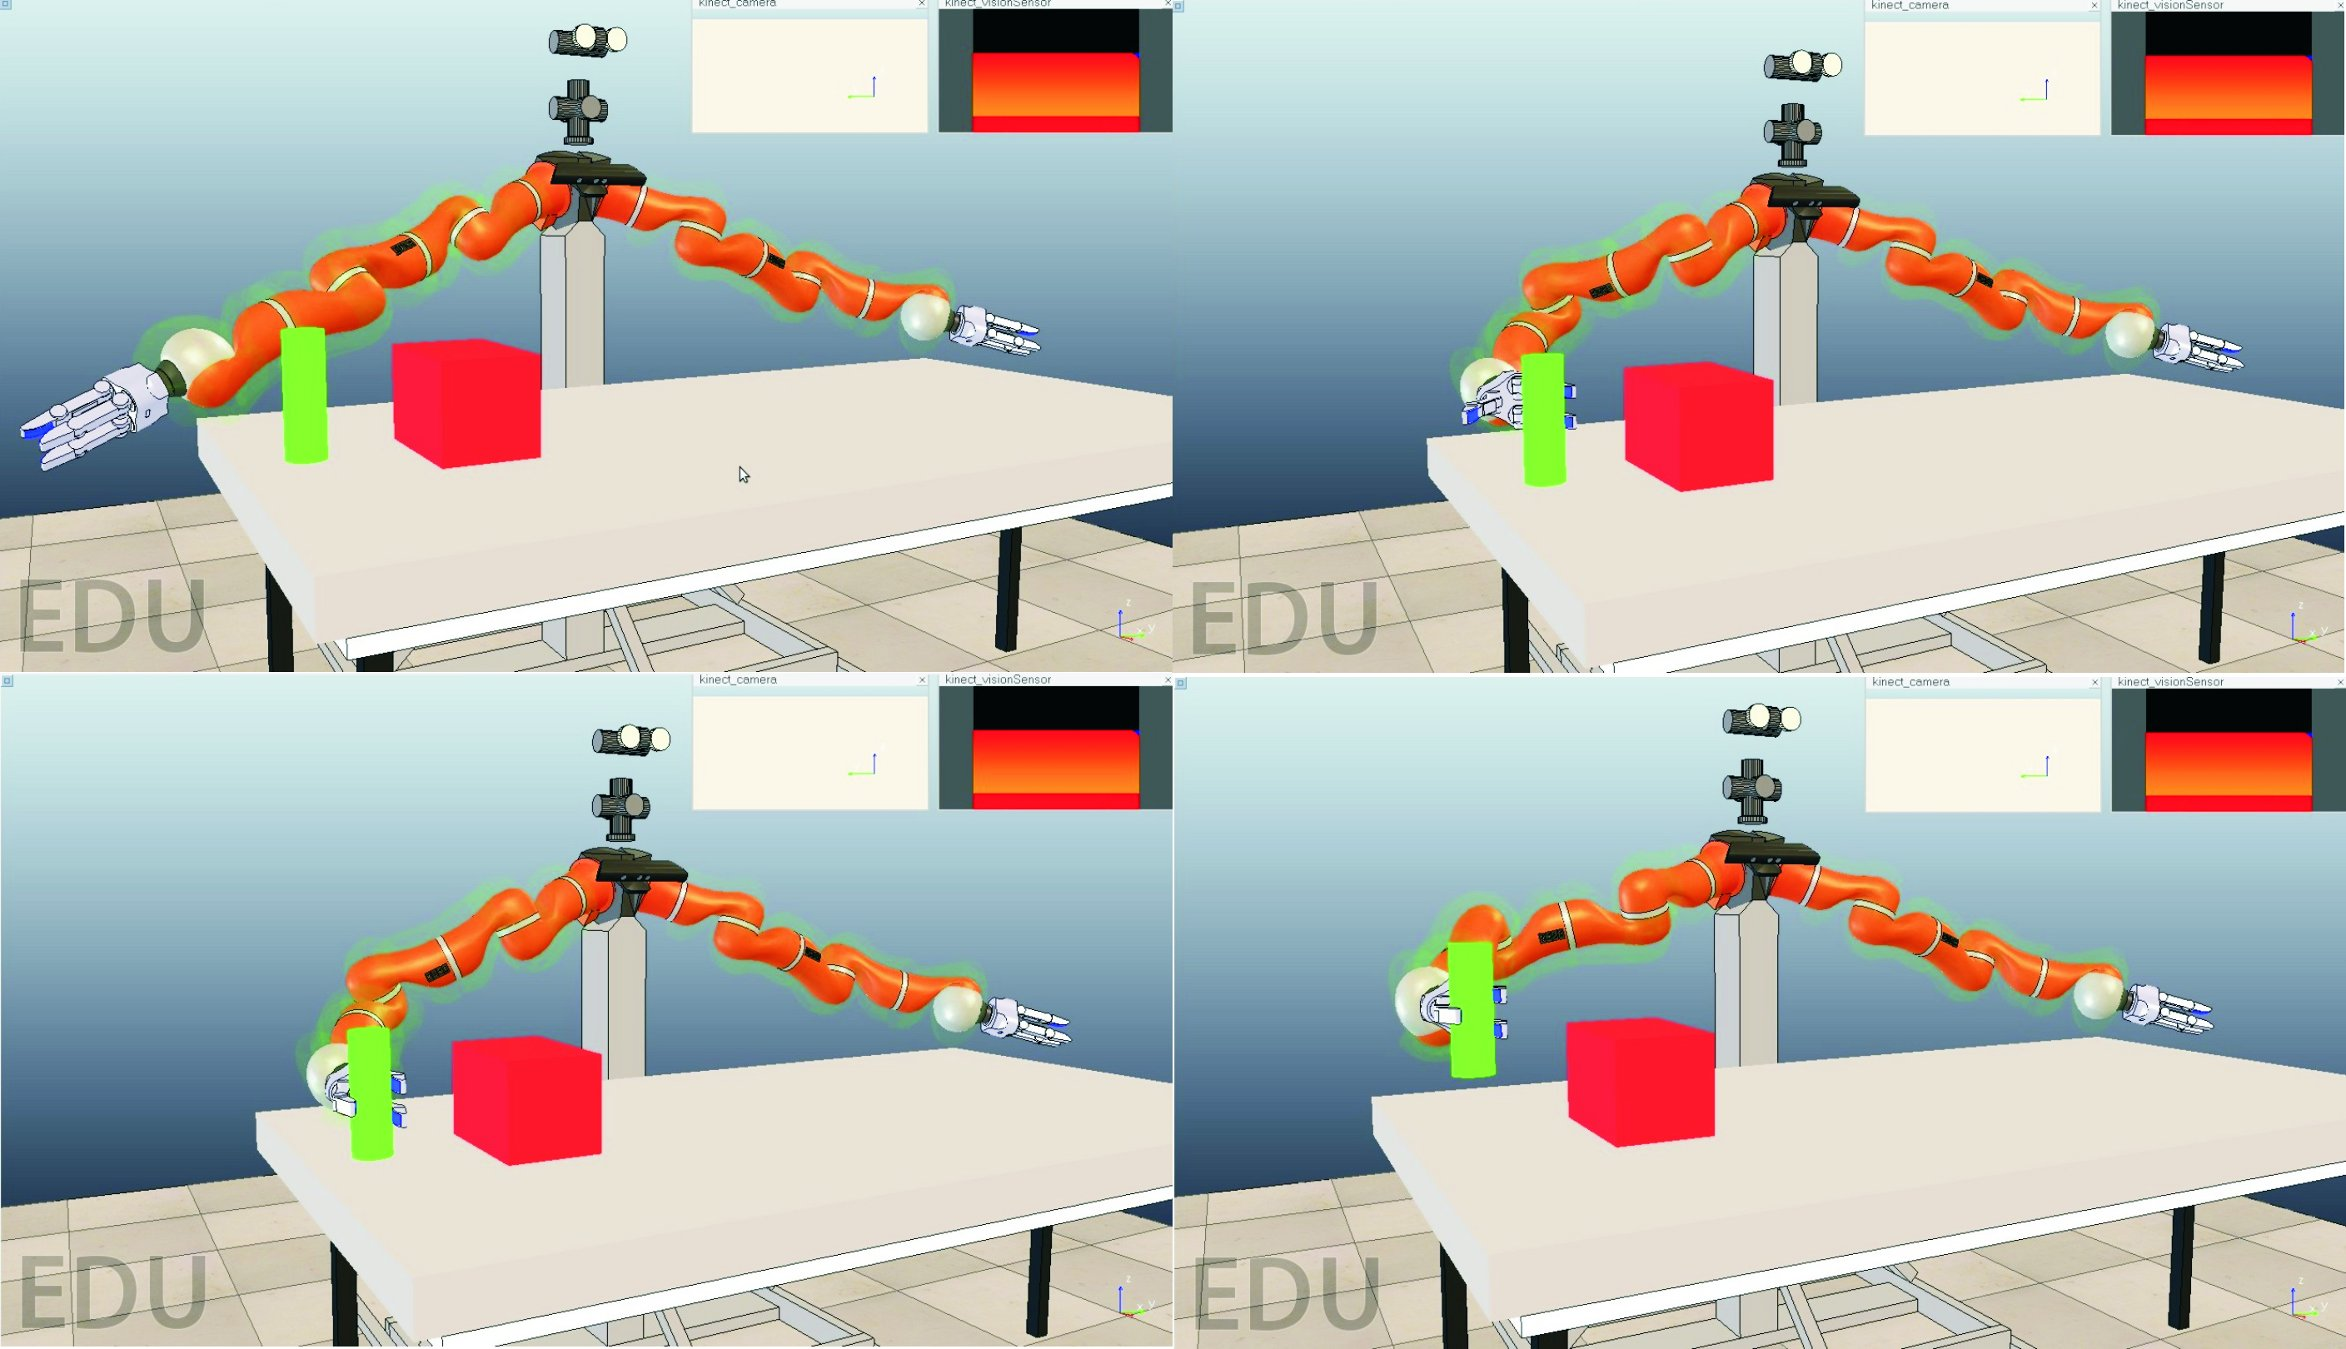
\includegraphics[width=0.75\textwidth]{images/pickup.jpg}
	\caption{Stages of the pickup phase in the simulator}
	\label{fig:pickup}
\end{figure}

\item \textbf{Placement phase} \\

The placement phase starts after a successful pickup. The grasped object is enclosed by the gripper and considered to be part of the robot. Now the manipulator moves towards the \emph{pre-place location} - the place where the final approach towards the goal starts. The easy way is to just drop the object at that point. In that case, the placement phase completes after bringing the gripper fingers into the \emph{post-place posture} (opening it) and detaching the object from the robot.

If the object should to be placed carefully, the gripper has to approach from the \emph{pre-place location} towards the final \emph{place location} along the specified approach direction. Here has to be considered that the object will get into contact with the support surface again when it's final position is reached. At that stage the gripper can open and the object has to be detached from the robot. From that point, the object needs to be treated as obstacle again which means the planner is forced to avoid collisions with it. The placement phase completes after the manipulator has moved away from the object along the specified retreat direction. The stages of the placement phase can be seen in Figure \ref{fig:placement}.

\begin{figure}[ht]
	\centering
  	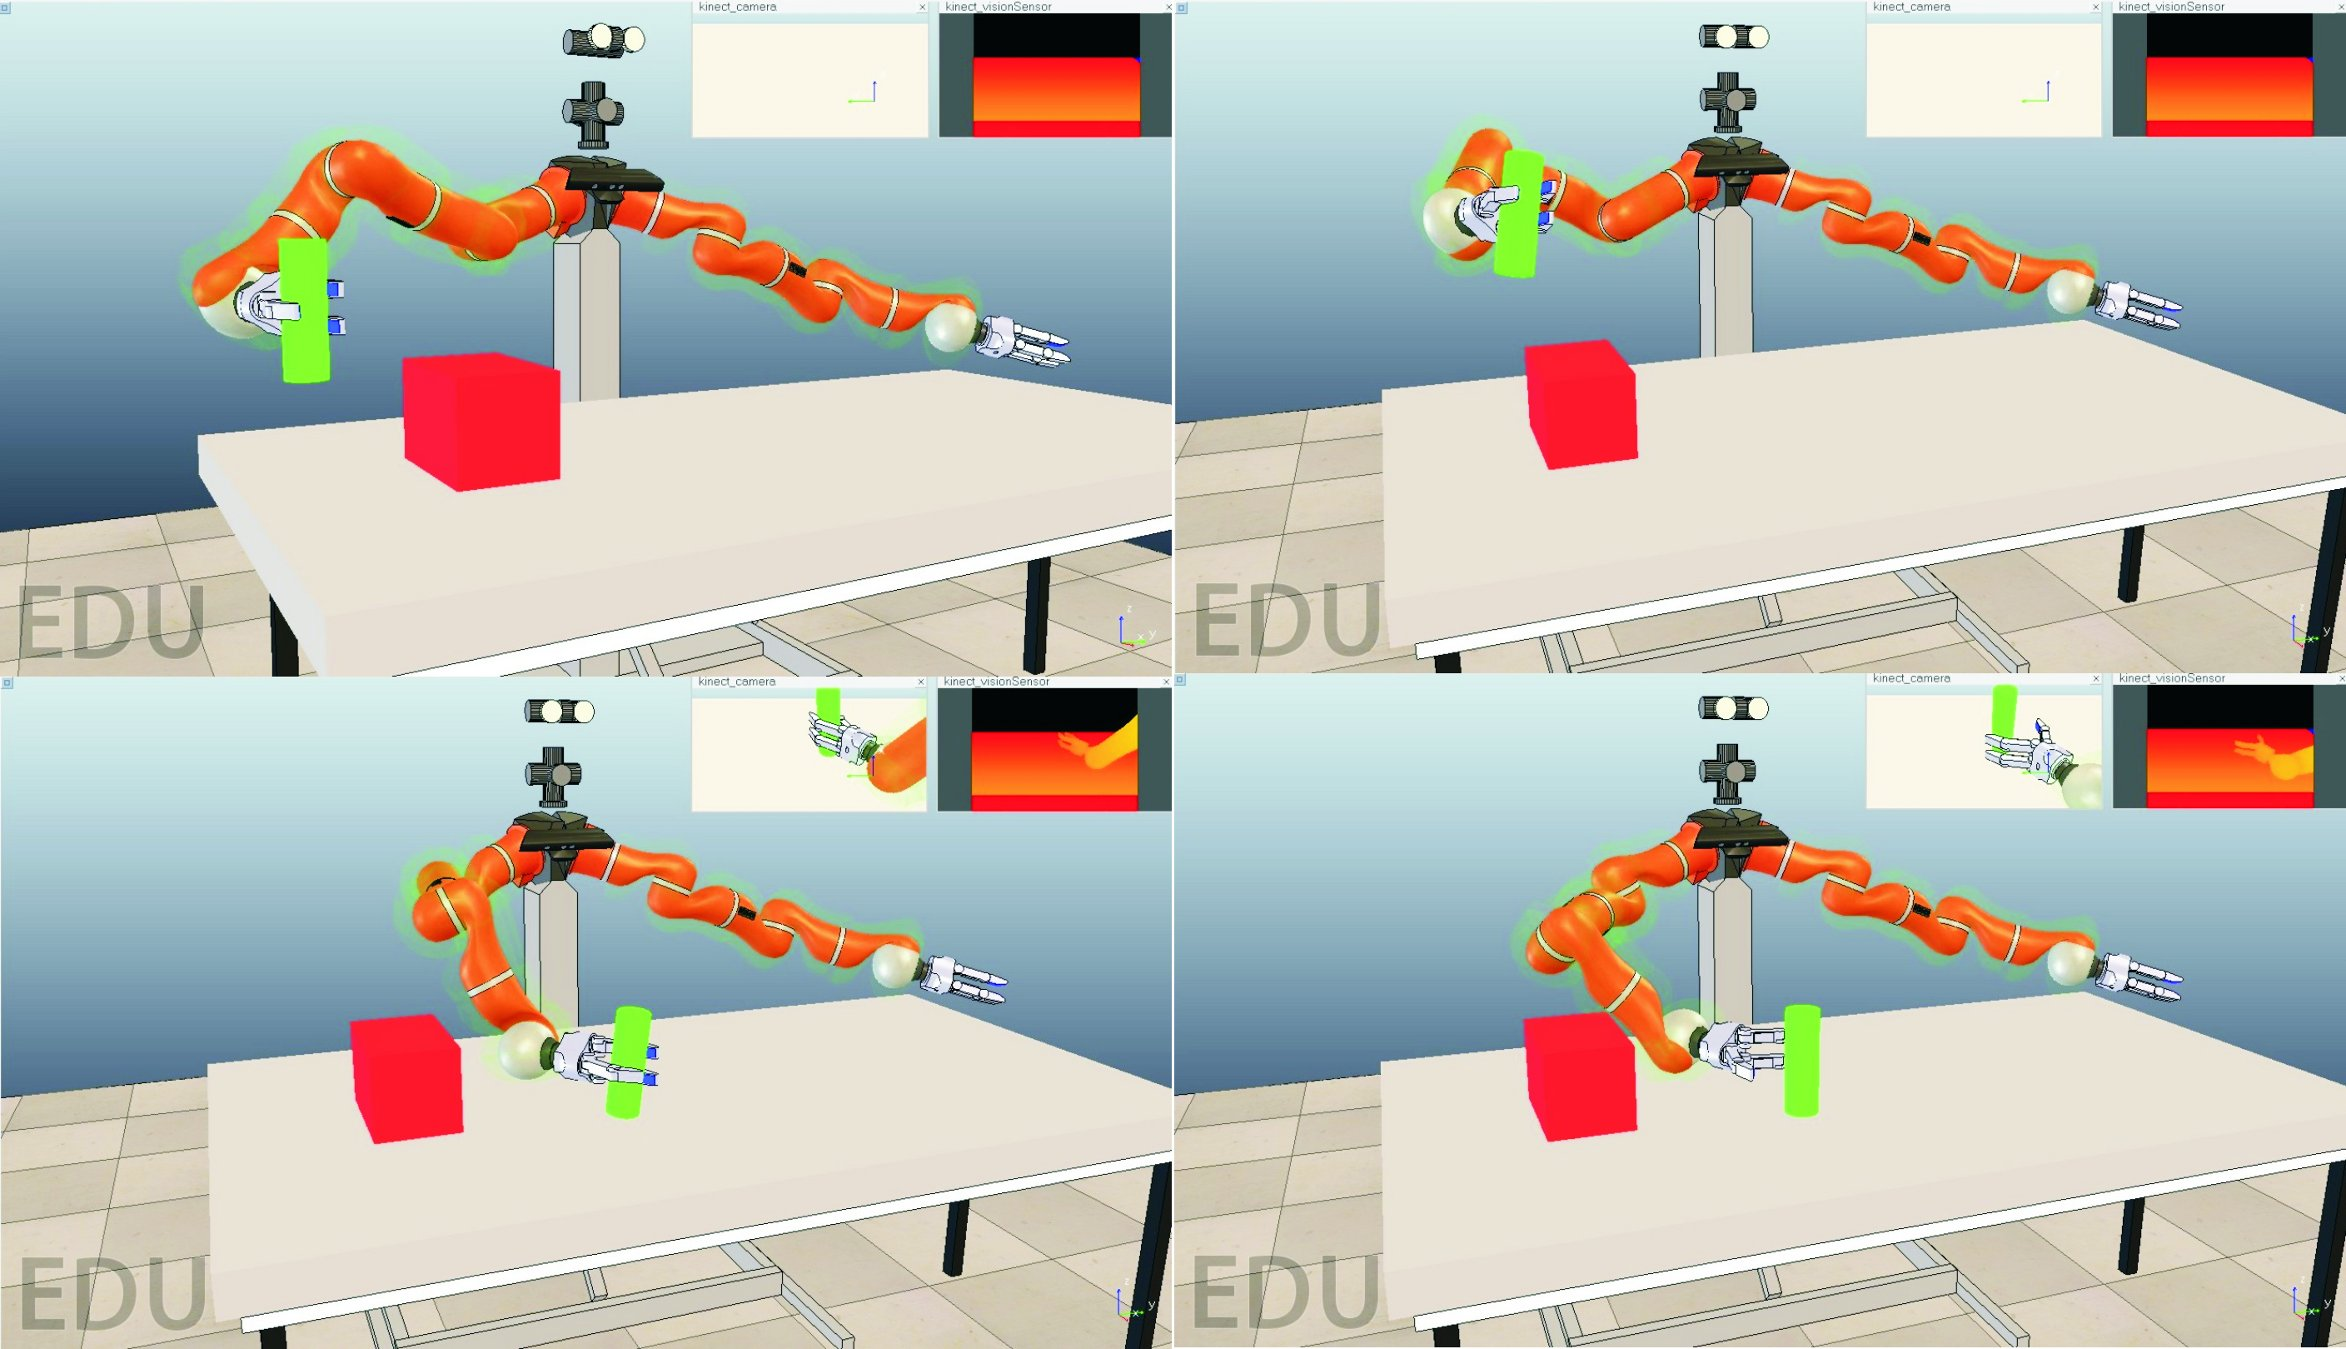
\includegraphics[width=0.75\textwidth]{images/placement.jpg}
	\caption{Stages of the placement phase in the simulator}
	\label{fig:placement}
\end{figure}

\end{itemize}

Both phases of the task are only considered to be complete if each single stage has successfully been executed. The necessary planning parameters like pre-grasp and grasp pose, gripper postures and approach and retreat directions are usually provided by a \emph{grasp planner}. This is an additional node within the planning pipeline that identifies objects in the environment of the robot, usually based on 3D sensor data and calculates the necessary grasp parameters. Explaining the functionality of grasp planners is far beyond the scope of this project though the section about implementing the reference task discusses the used parameters in greater detail and shows what would be usually delivered by the grasp planner.


\section{Pick and place tasks in MoveIt}

During the various stages of the pickup and placement phases a lot of motion planning is required. Each single stage requires to plan a trajectory that is free of accidental collisions while respecting the limits of the robot and enforcing possible additional constraints. Each phase can only be considered executable if a valid motion plan for each single stage exists. Planning all the subsequent stages one after the other would be a cumbersome task. Therefore MoveIt provides a set of messages and action servers that greatly simplify those planning tasks.\\

The \emph{PickupAction} server handles the planning and optionally execution of all required stages during the pickup phase at once. Pickup requests are done, using a \emph{PickupAction} client to send \emph{PickupGoal} messages to the server. The request message is composed of all the parameters that are necessary to completely describe the planning problem. Picking up an object can always be done in several ways. Depending on the shape of the object there hardly always exist a lot of possible poses where the gripper can safely approach and grasp. Therefore MoveIt allows to provide a set of possible grasp definitions for a pickup request. There is also a quality parameter that can be used to tell the planner, how `good' a specific grasp is compared to other ones. MoveIt can then favour grasps with higher quality if several valid solutions are found by the planner. Providing a number of different grasps increases the probability for the request to be successful. The grasp definition is composed of the pre- and post grasp postures for the gripper, the final grasp pose and the approach and retreat vectors. As MoveIt needs to know which object should be picked within the planning scene, it is also necessary to include the ID of the object to grasp.\\

The \emph{PlaceAction} server is responsible for planning the whole placement phase. Therefore same concept is used as above - a set of possible place locations can be provided to increase the probability of a successful planning attempt. The parameters that are used to describe a place location include the post-place posture of the gripper along with it's target pose, and vectors, describing the pre-place approach and the post-place retreat.\\

Pickup and placement requests as well require a number of additional parameters that are explained in greater detail within the section about benchmark task implementation. 

Objects contained in the task environment have to be brought to MoveIt's attention. This can be done either by manually adding them to the planning scene, using the corresponding topics or by configuring MoveIt to be aware of sensor data. As the integration of depth information from the Kinect camera did not work stable during the evaluation phase, that possibility is not covered within this thesis and all involved objects were added manually.

Pickup- and place action servers provide the ability to choose whether to execute motion plans immediately or to do just the planning and return the outcome. In that case the execution has to be handled manually later on. 
The first method is much more comfortable as MoveIt executes the trajectories and also handles additional requirements like attaching and detaching the grasped object in time. The drawback is that also possibly weird trajectories get executed immediately as they might be valid solutions for the given planning problem though they are obviously unsuitable. So an additional safety mechanism needs to be introduced that allows to interrupt the execution when facing any problems.
The second method allows to visualize the resulting trajectories and then decide whether to execute them or not. But then each single trajectory stage has to be executed manually which also includes attaching or detaching objects to the manipulator. The advantage of this method is the clean separation between planning and execution, allowing maximum control over the execution flow. Therefore this method was favoured during benchmark task implementation.

\section{Implementation of the benchmark task}

This section describes the implementation of the benchmark pick and place task in greater detail. The source code can be found within the `uibk\_moveit\_tests' package. The workspace is the table in front of the robot covered with a 9cm thick foam mat. This mat will be declared as the support surface later on. The object to grasp is a cylinder with 4cm radius and a height of 25cm. This corresponds to the size of a usual SIGG bottle which can be used to run the benchmark task in the real world. The cylinder is located on a fixed, known position. There is also a box shaped object located within the workspace that acts as an additional obstacle. The goal of the task is to pick the cylinder up, using the right arm of the robot and place it at the goal location without colliding with the obstacle or other parts within the robot's environment. The implementation makes use of MoveIt's pick and place functionality. The necessary steps are explained in the following subsections.

\subsection{Creating the environment}

As MoveIt is currently not configured to use sensor data, it has to be notified about the task environment. The table and the surface mat are already part of the URDF description but the cylinder and the obstacle have to be added to the task environment. This is done utilizing the \texttt{planning\_interface::PlanningSceneInterface} class that provides functionality to manipulate the current planning scene. The same effects can be achieved by manually publishing to the `/collision\_object' topic but using the convenience class saves a lot of boilerplate code. The \emph{CollisionObject} type is used to describe those objects. Both of them are primitive shapes. Necessary parameters are the shape type, dimensions and the target pose. Additionally each \emph{CollisionObject} needs a unique ID which is used to identify the shape within the planning scene. After adding the \emph{CollisionObjects} to the collision world, they are visualized in RViz. The image in Figure\ref{fig:task_env} shows the task environment after adding the \emph{CollisionObjects}.

\begin{figure}[ht]
	\centering
  	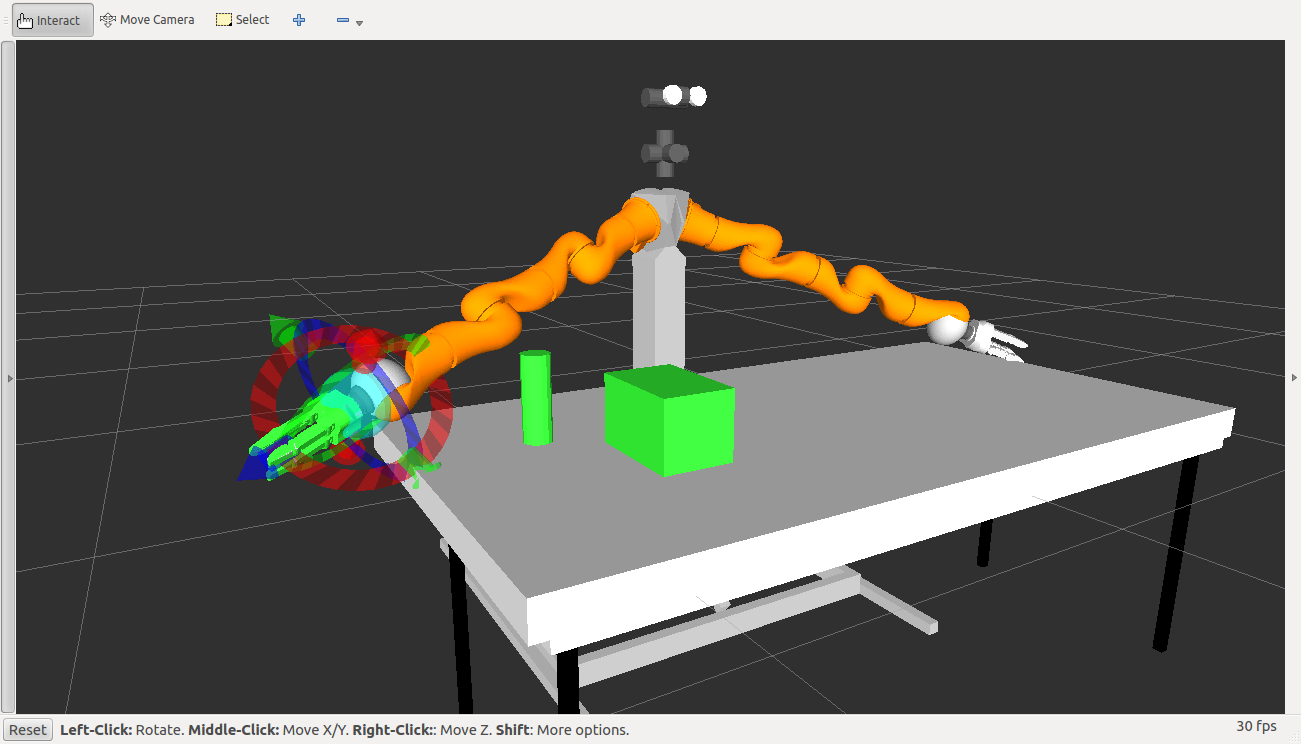
\includegraphics[width=0.75\textwidth]{images/task_env.png}
	\caption{Planning scene after inserting the collision objects}
	\label{fig:task_env}
\end{figure}

\subsection{Generating possible grasps}

Before calling the pickup action server it is necessary to generate a set of possible grasps for the object to pick. This information is usually provided by a grasp planner. The sample task encapsulates the grasp planner functionality within the \emph{generateGrasps} method. This method takes the current pose of the cylinder as input parameter and calculates 10 possible grasp poses along a semi circle around the cylinder location. Pre-grasp and grasp postures are joint trajectories for the gripper, containing just one trajectory point stating the target configuration for the gripper in the opened respectively the closed state. The pre-grasp approach and the post-grasp retreat are defined as \emph{GripperTranslations}. This is a special message type that describes the direct gripper movement from one position towards a target. The direction is defined as a three dimensional vector. The length of the translation can be set in a flexible way by specifying a desired distance and a minimum distance. Experiments showed that the success rate is much better if the grasp parameters allow some flexibility to the planners. The approach vector depends on the grasp pose and points along the z-axis of the end effector frame towards the object. The desired distance between pre-grasp and grasp pose is set to 20cm while the minimum distance is 10cm. The gripper retreat vector points up, along the z-axis of the world. Desired and maximum distances are also set to 20cm respectively 10cm. As no one of the generated grasps should be favoured among the others, the grasp\_quality parameter of each grasp is set to 1. This means that they are equal in quality. The last necessary parameter is a unique identifier for each grasp. As usually a lot of different grasps are provided for each pickup request, this ID can be used to identify, which one was finally used to solve the planning problem.

\begin{figure}[ht]
	\centering
  	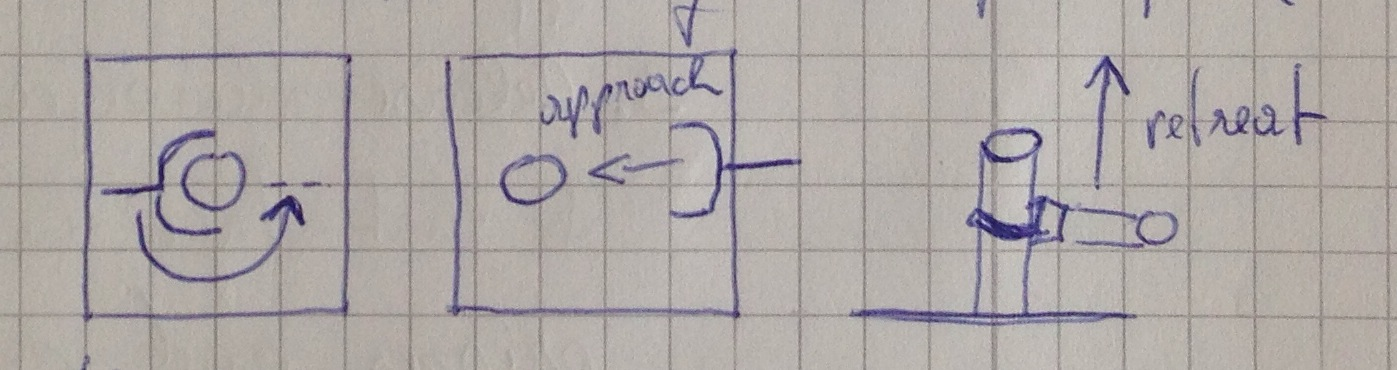
\includegraphics[width=0.75\textwidth]{images/grasp_stages.jpg}
	\caption{Grasp poses, gripper approach and retreat}
	\label{fig:grasp_stages}
\end{figure}

\subsection{Planning and executing the pickup}

After generating the set of grasps, the planning request can be sent to the pickup action server. As there is a lot of boilerplate code necessary, a reusable helper class was created that can be used to simplify all kinds of planning requests. The utility class is called \emph{PlanningHelper} and can be found within the 'uibk\_planning\_node' package. A call to the pickup action server is done by using the `plan\_pick' method of the helper class. This method takes a set of possible grasps and the ID of the object to pick as parameters. The outcome is a pointer to an instance of \emph{PlanningResult}, a structure that contains all the necessary information about a planning attempt. Success or failure is indicated by the `status' parameter. On success, the parameter `trajectory\_stages' holds a vector, containing the resulting trajectory stages. The actual call to the pickup action server is done by defining the  \emph{PickupGoal}, using the predefined grasps. Additional parameters are the ID of the object to pick, the name of the chosen planning group and the name of the link within the robot model that acts as the support surface. Optional parameters are among others the ID of the planner to use and the maximum allowed planning time. The parameter `plan\_only' within the planning options is set to true to avoid the immediate execution of the planned trajectories. This allows a visual verification of the planning outcome before execution. The resulting robot path is shown in RViz. If the solution is satisfying it can be executed, passing the PlanningResult to the corresponding method of the PlanningHelper class. This method uses the `/execute\_kinematic\_path' service provided by the `move\_group' node. The service sends a given trajectory to the responsible controller and provides feedback information about the execution status. The `PlanningHelper' also takes care to attach the picked object to the gripper after the grasp stage. The pickup phase completes after successful execution of all trajectory stages.


\subsection{Planning and executing the placement}

The placement phase is planned and executed in a somehow similar manor. The cylinder has to be placed on a specific location within the workspace in an upright position - the rotation around the z-axis doesn't matter. Therefore a set of possible place poses is generated in 20 different orientations around the z-axis. This again gives some freedom to the planner as it can choose which one to use (TODO: provide image that shows the principle). The final approach towards the goal location is specified as \emph{GripperTranslation}. The direction vector points down along the z-axis of the world. Desired and minimum distances are set to 20cm respectively 10cm, allowing some flexibility during that stage. As post-place posture for the gripper, the same configuration is used as for the pre-grasp posture. The last required parameter for a place location is the \emph{GripperTranslation} that describes the retreat after releasing the object at the goal location. The direction depends on the chosen orientation and points towards the negative z-axis of the gripper reference frame. 

\begin{figure}[ht]
	\centering
  	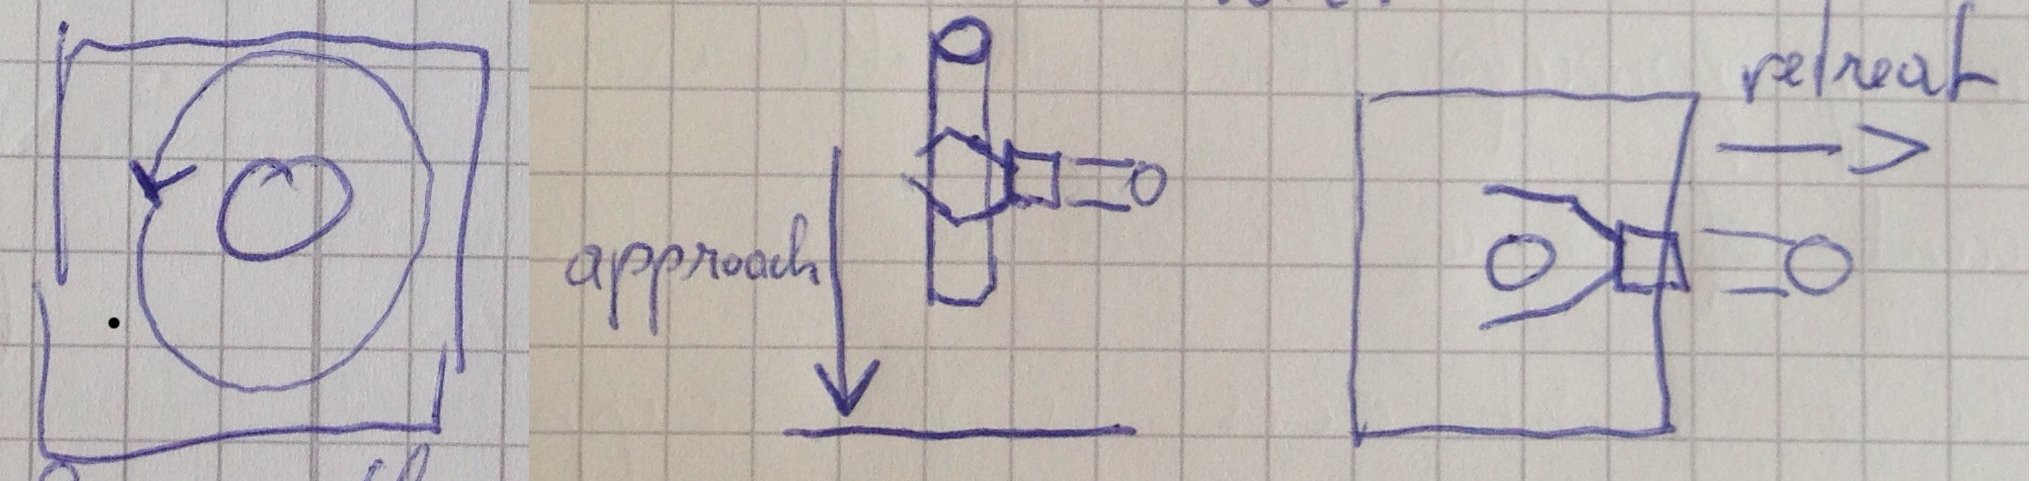
\includegraphics[width=0.75\textwidth]{images/place_stages.jpg}
	\caption{Place locations, pre-place approach and post-place retreat}
	\label{fig:place_stages}
\end{figure}

The call to the place action server is again handled by the formerly mentioned planning helper class. The `plan\_place' method takes a vector of the predefined place locations and the ID of the object to place as input parameters. The actual call to the place action server is done, defining a \emph{PlaceGoal} message. The most important parameters are the ID of the object to place, the name of the planning group and the set of possible place locations. Optionally can be specified which planner to choose and also the maximum allowed planning time. The method returns the result of the planning request. On success, the resulting trajectories are again visualized in RViz and can then be executed the same way as during pickup phase. After the execution, the task is considered to be complete and the picked object is detached from the gripper and again part of the collision world.


\section{Executing the benchmark task}

The benchmark task is designed to run on the simulator and the real robot as well. The sample program only depends on a running `move\_group' instance. The easiest way to run the sample is to start MoveIt in demo mode (demo.launch) and then execute the sample code, using.

\begin{verbatim}
rosrun uibk_moveit_tests sample_pick_place 
\end{verbatim}

This demonstrates the functionality but only executes the trajectories on the fake controllers provided by MoveIt. If the sample should be executed on the simulator or the real robot, the corresponding namespace has to be specified before running the code. This can be done by setting the `ROS\_NAMESPACE' environment variable to either `simulation' or `real', within the terminal. For example

\begin{verbatim}
export ROS_NAMESPACE=simulation
rosrun uibk_moveit_tests sample_pick_place 
\end{verbatim}

runs the benchmark task on the simulator. Of course it is necessary to start the simulator and launch the corresponding MoveIt instance before doing that. After creating the environment and adding the objects to the planning scene the pickup phase gets planned. The outcome can be seen in RViz and the program will ask if the resulting trajectory is ok and should be executed. A negative answer will force the program to replan the pickup and ask again, otherwise the trajectory gets executed. After successful execution, the place phase gets planned. The resulting plan also is the visualized as well and execution needs confirmation again. The program exits after successful completing the placement phase.

\section{Observations}

This section gives an overview about the most important observations that have been made during the implementation of the sample task:

\begin{itemize}

\item

It is very important to provide some degree of freedom to the planner at various points. Major points are the amount of different grasps or place locations and the allowed range within the defined gripper translations. Very strictly defined planning requests are very likely to fail whereas requests with a higher degree of flexibility drastically raise the overall success rate.

\item

Working with path constraints drastically drops the success rate because the high complexity of the planning problem. Enforcing path constraints requires much more allowed planning time and a very fast IK solver because of the large number of necessary IK requests. Maybe a faster IK solution than the one available could help to solve the problem but that is not guaranteed. Therefore there are no path constraints used within the sample task.

\item

Planning requests often fail due some MoveIt-internal issues and not because planning is not possible at all. Therefore it is necessary to repeat failed requests because it is very likely that planning succeeds on subsequent attempts. In the sample task implementation, the planning requests are done within a loop. If a request fails, it gets repeated. A successful request breaks the loop and continues the execution flow.

\item

Resulting trajectories should always be visualized in RViz before confirming the execution. The calculated motion plans might be valid but sometimes they are a bit confused and therefore unsuitable. Moreover, the planner can only take into account what it knows about the robot's environment. Especially in the robot lab there is equipment mounted in the area above the robot, that is not taken into account during planning. Therefore the visual validation is necessary to avoid damages on the robot and it's environment.

\end{itemize}

%\lstset{language=C++}
%\begin{lstlisting}

%This is code

%int a = 0;
%printf("Dies ist ein Test");

%\end{lstlisting}

%\lstinputlisting[language=C++,
%				 directivestyle={\color{black}},
%				 emph={int,char,double,float,unsigned},
%				 emphstyle={\color{blue}}
%				]{code/move_goal.cpp}




